% !TeX root = ../document.tex
\documentclass[../document.tex]{subfiles}
\lstset{inputpath=sections}
\begin{document}	
	\subsection{The basics of decision trees}
	Basically, tree-based methods segment the predictor space into a large number of simple regions. The prediction for a test sample is based on findig the appropriate region to which the test sample belongs.
	\paragraph{Regression trees}
	
	\paragraph{Prediction via stratification of the feature space}
	There are two steps necessary to build a regression tree. 
	\begin{itemize}
		\item The predictor space needs to be divided into non-overlapping regions \(R_{1},...,R_{j}\)
		\item For every observation that falls into the region \(R_{j}\), we make the same prediction
	\end{itemize}
	The focus is on dividing the predictor space into high dimensional rectangles (boxes). Hence the goal is to find boxes that minimize the RSS.
	\begin{equation}
		RSS = \sum_{j=1}^{J}\sum_{i\in R_{j}}(y_{i}-\hat{y}_{R_{j}})^2
	\end{equation}
	Unfortunately this problem cannot be solved in general optimally within a reasonable amoutn of computation effort. Hence a top-down, greedy approach that is known as recursive binary splitting is used.\
	First te predictor \(X_{j}\) and the cutpoint s is selected such, that splitting the predictor space into the regions leads to the greatest possible reduction in RSS. Hence we need to consider all possible predictor variables and all possible cutpoint values for each of the predictor variables to make the best greedy decision. But note, no combination of predictor variables are considered, hence the "stratification" of the feature space.\
	Once the root has been split into two regions, the same procedure is applied recursively to the newly generated regions until a stopping criterion is reached.
	\begin{center}
		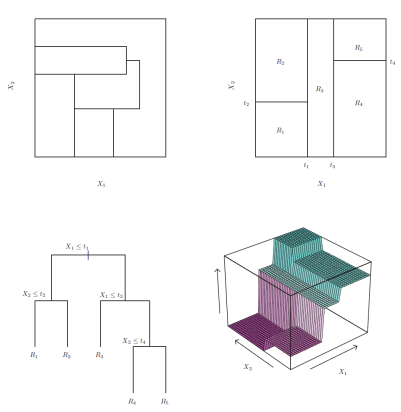
\includegraphics[width=.6\textwidth]{pictures/tree.png}
	\end{center}
	\paragraph{Tree pruning}
	The presented procedure, without modification, would result in low training MSE but probably high test MSE, since the tree is allowed to be quite complex. Better, we grow a very large tree and then prune it down to a small one.\
	We would like to select the subtree, which results in the lowest test MSE. Cost-complexity pruning is an elegant way to find these candidates.\
	We use the number of terminal nodes |T| as a measure of the flexibility of a particular tree. As before (lasso), when we want to control the number of regions (coefficients), we add a penalty term to the RSS minimization problem.
	\begin{equation}
		\sum_{m=1}^{|T|}\sum_{x_{i}} \in R_{m}(y_{i}-\hat{y}_{R_{m}})^2 + \alpha|T|
	\end{equation}
	Now the tuning parameter \(\alpha\) control the trade-off between RSS reduction and complexity of the tree. As \(\alpha\) increases, the tree become simpler. We find the best tuning parameter with cross validation.
	\paragraph{Classification trees}
	Classification trees predict qualitative responses instead of quantitative ones. A classification tree can also be grown using recursive binary splitting. A extension is, to split in such a way that we maximize the reduction in classification error rate.
	\begin{equation}
		E = 1-max(\hat{p}_{mk})
	\end{equation}
	This error rate is simply the fraction of the training observations in a region m that do not belong to the most common class, but this isn't sesitive enough. An alternative is the gini index.
	\begin{equation}
		G = \sum_{k=1}^{K}\hat{p}_{mk}(1-\hat{p}_{mk})
	\end{equation}
	The gini index is a measure of total variance across the K classes in the region m. It is small if one of the proportions are close to one and all the others are close to zero. Hence it is a measure of node purity, a low number implies a pure node.\
	The cross-entropy of a region m is defined as follows:
	\begin{equation}
		D = -\sum_{k=1}^{K}\hat{p}_{mk}log\hat{p}_{mk}
	\end{equation}
	If all classes are about equally likely the uncertainty is high and if one class dominates, the uncertainty is low.
	\paragraph{Trees vs. linear models}
	If the relationship is well approximated by linear model, then linear regression works well. If the relationship is highly non-linear and complex then cecision trees might outperform classical approaches. Trees are very easy to explain to people and some people believe that decision trees more closely mirror human decision-making than the regression and classification approaches in the previous chapters. Trees can be displayed graphically and can easily handle qualitative prodictors without the need to create dummy variables. But trees generally do not have the same level of predictive accuracy as some ot the other approaches.
	\subsection{Bagging, random forests}
	\paragraph{Bagging}
	Decision trees suffer from high variance. Bootstrap aggregation (bagging) is a general method for reducing the variance of a statistical learning method. Recall that averaging a set of n independent observations with equal variance will result in a sample mean that has a variance that is n times smaller than the variance of each sample.
	Since we have not multiple training sets, we can bootstrap. 
	\begin{equation}
		\hat{f}_{bag}(x)=\frac{1}{B}\sum_{b=1}^{B}\hat{f}^{*b}(x)
	\end{equation}
	Bagging can improve prediction for many regression methods and its particularly useful for decision trees. But bagging can also be used for classification problems. The decision of the single trees cannot be averaged, but one can use the most commonly occurring class among all trees as the final class prediction.
	\paragraph{Random forests}
	Random forests use an elegant trick that decorrelates the trees, which improves on the performance of bagging. As in bagging, the decision trees are built using bootstraped training samples, but for every split a random sample of m predictors is chosen as split candidates. Typically m=sqrt(p). Hence for each split, only a random majority of possible predictors are evaluated.\
	If there is a strong predictor in the data set, most trees would use this one as the top split. Hence the bootstrapped trees all look quite similar, which means their predictions are correlated, which means averaging them will not improve matters much. But with breaking this structure by only allowing m randoly selected predictors, the averaging can be much better.
\end{document}